\section{讲解笔记：【第4次作业笔记】 梁和刚架(1)}
\begin{analysisbox}
本节按题目、答案和讲解笔记顺序整理。对扫描图中的结构几何关系，正文保留 OCR 可识别文字，并在图形页中保留清理后的题图，便于核对杆件、支座、荷载和尺寸。
\end{analysisbox}
\subsection*{第 1 页转写}
结力基础班第4次作业-

梁和刚架

梁和刚架作业及答案

2-1图2-60所示结构截面A的弯矩（以下侧受拉为正）是（B

）。（西南交通大学

2008)

A. M

B. -M

C.-2M

D. 0

FoE=0, FcD=0

FPE

MA

图2-60

2-2图2-61所示结构剪力FQBA=0

。（重庆大学2010)

FAY

EMe=0,F

图2-61

Fay-1=0

: Fay=0

FAN

M\&C
\begin{figure}[H]\centering
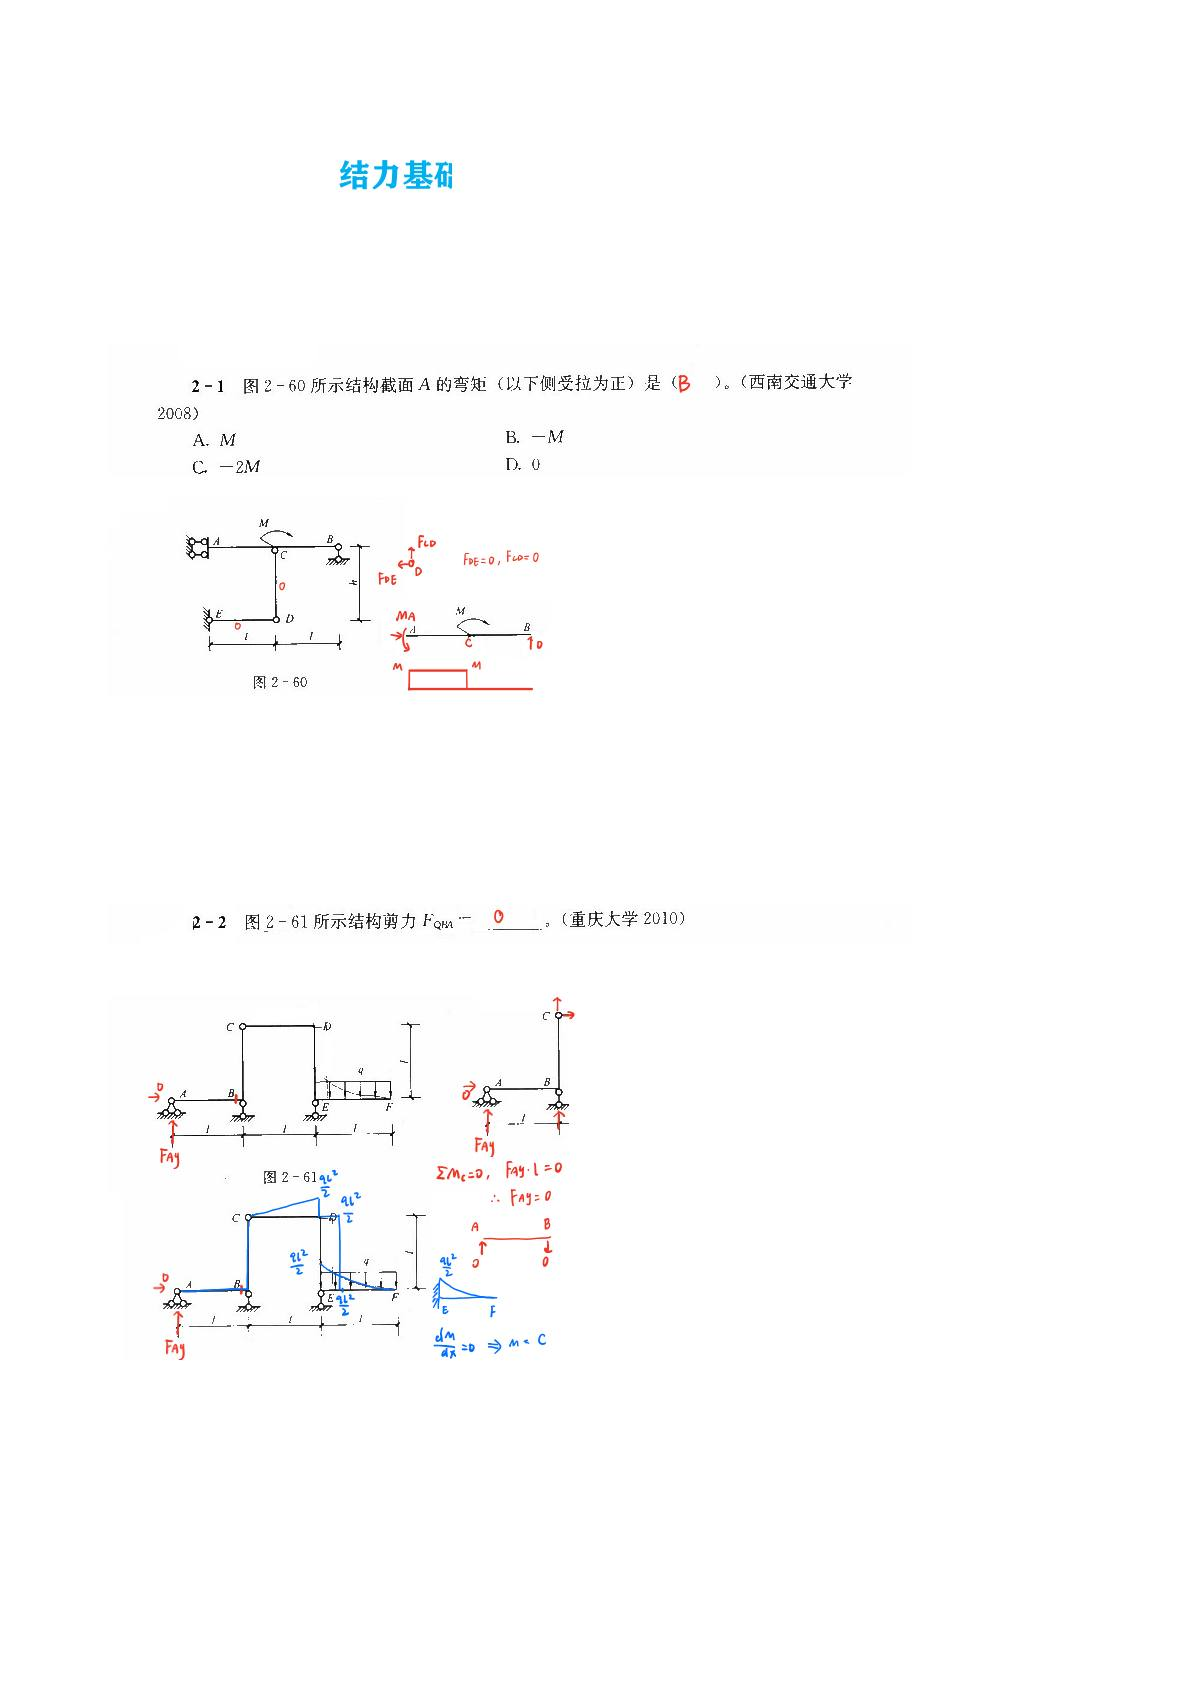
\includegraphics[width=0.92\textwidth]{figures/src24_p001.jpg}
\caption{【第4次作业笔记】 梁和刚架(1) 第 1 页清理图形页}
\end{figure}
\subsection*{第 2 页转写}
2-3

剪力为。（河北工业大学

2010)

10kN-m

30kN

4m

4x30$\times$4:30

5kN-m

8m

10kN-m

MAB

ghx ++ MAb - 80x 8-t=0

BBL

MAb: 3t W.y

5kN-m

8m

2m2m

10kN-m

B+es

30kN

SKN-

8m

2-4图2-63所示刚架，AD杆截面D弯矩M=-24

(内侧受拉为正)。（浙江

大学2011)

图2-63
\begin{figure}[H]\centering
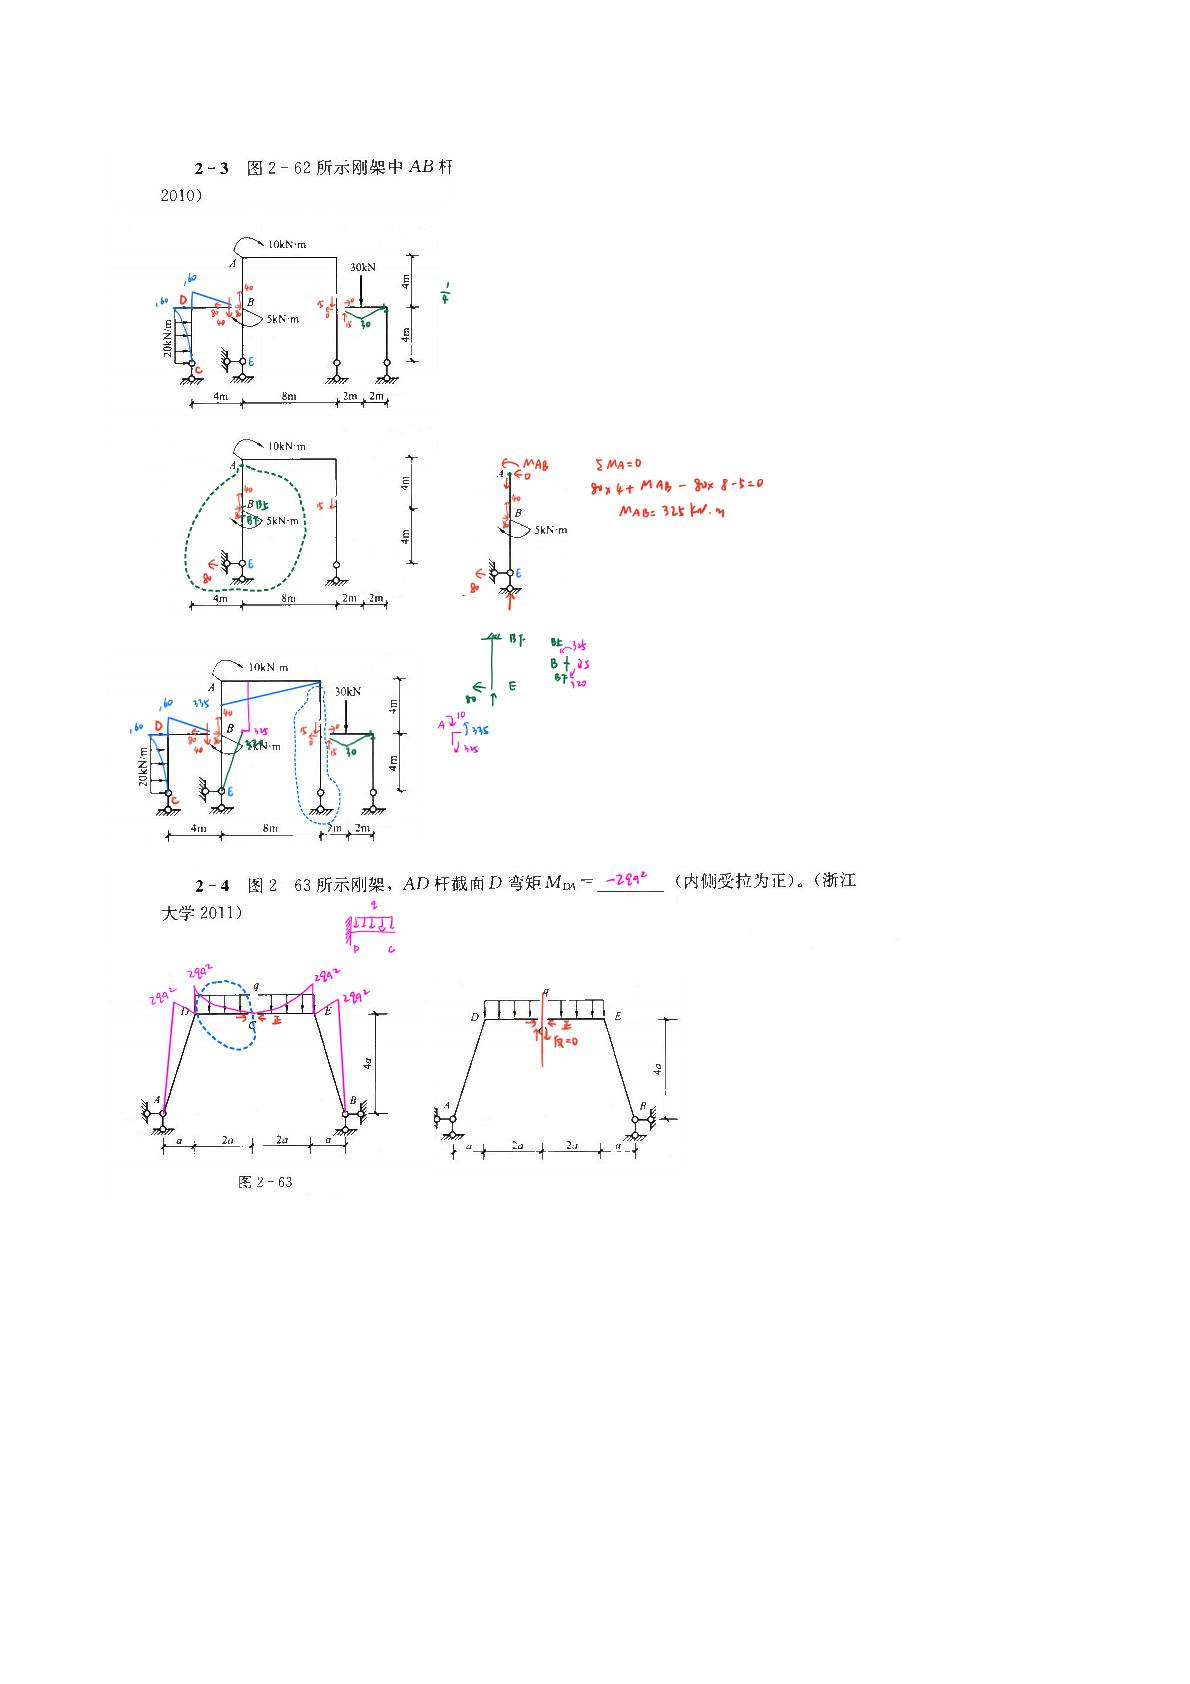
\includegraphics[width=0.92\textwidth]{figures/src24_p002.jpg}
\caption{【第4次作业笔记】 梁和刚架(1) 第 2 页清理图形页}
\end{figure}
\subsection*{第 3 页转写}
2-5试作图2-64所示结构的弯矩图。（北京科技大学2008）

4kN

10kN

10kN

6kN/m

4KN

6kN/m

图2-64

认为4kn在B铰左边

10kN

4kN

6kN/m

+xb233

YF

49

IMp =0

TFyF-9

认为4kn在B铰右边

10kN

6kN/m

PF

2-6作图2-65所示多跨梁的弯矩图和剪力图，并给出AB杆的受力平衡图。（北京

交通大学2011)

20kN

10kN/m

20kN

40kN-m

40kN-m

10kN/m

8$\times$2m

8x2m

$\alpha$二0, m=常数

图2-65

20kN

，m科直

40kN

10kN/m

DAYD

8$\times$2m

20kN

40kNm

10kN/m

8$\times$2m
\begin{figure}[H]\centering
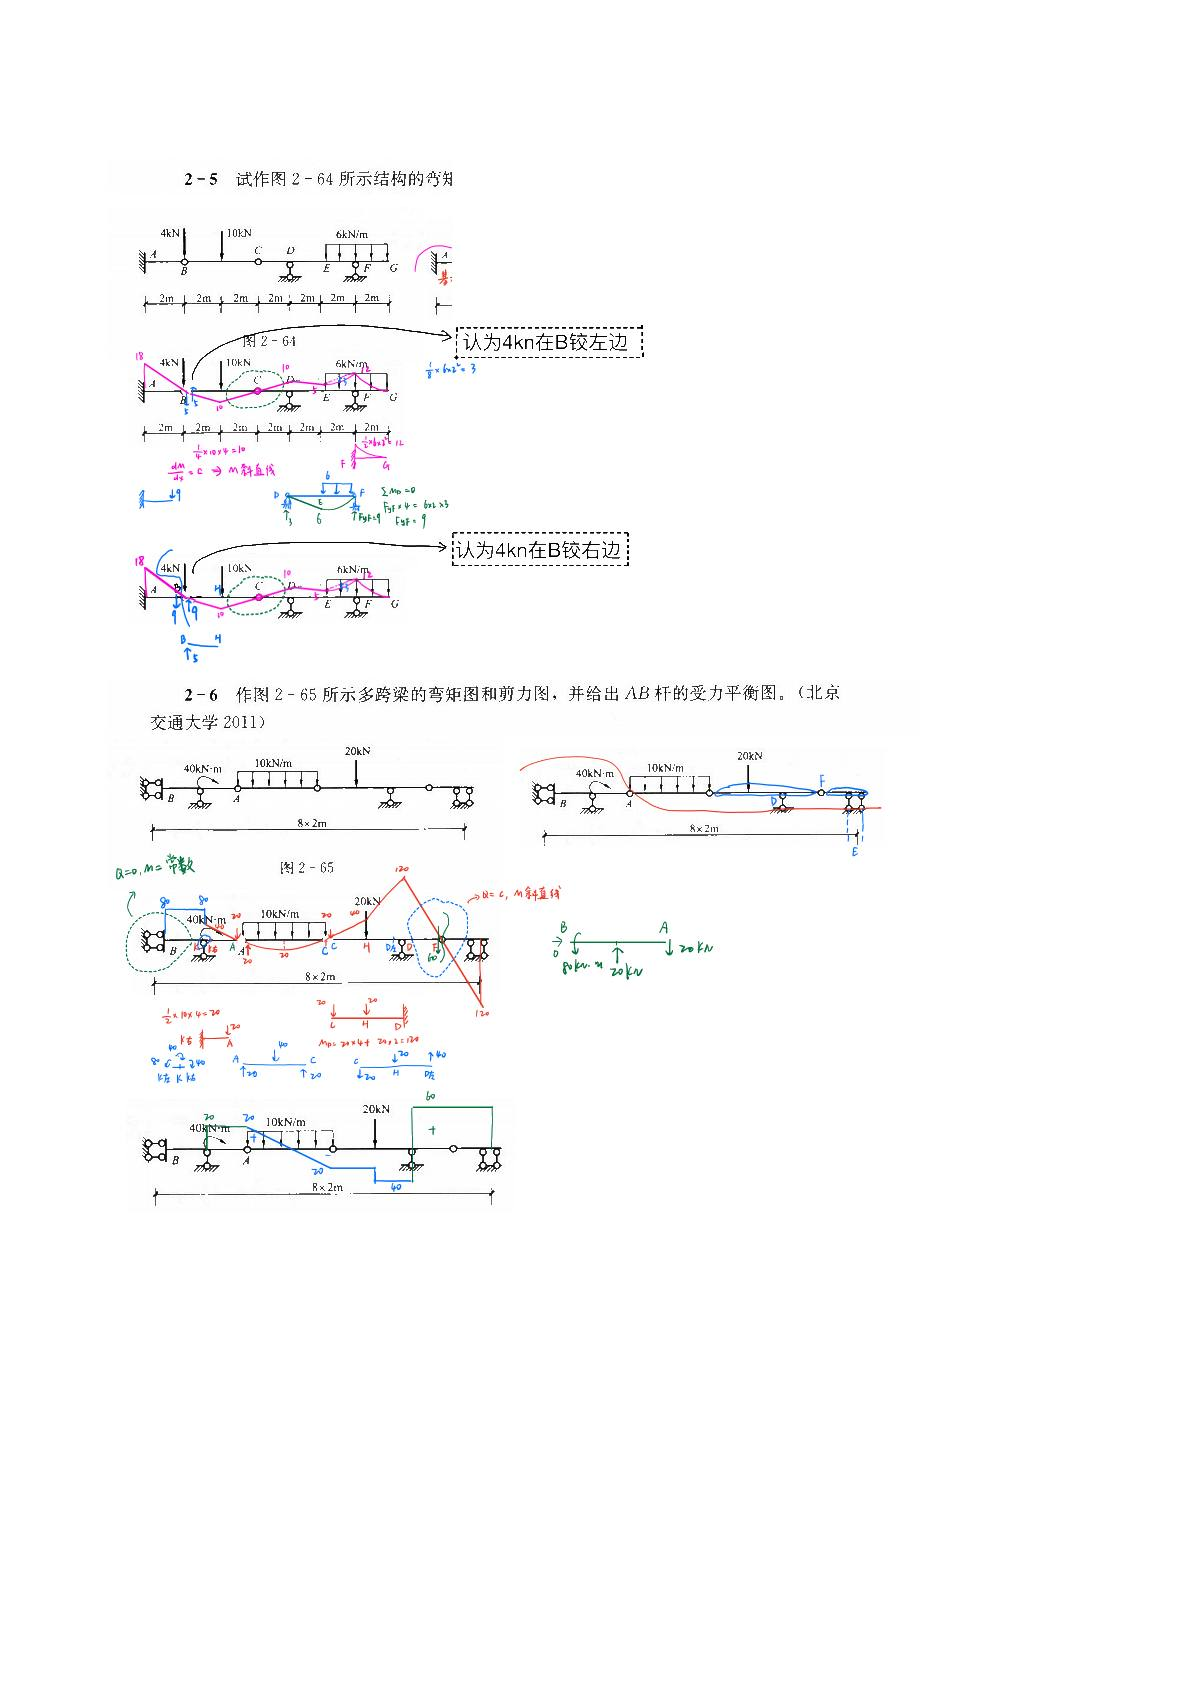
\includegraphics[width=0.92\textwidth]{figures/src24_p003.jpg}
\caption{【第4次作业笔记】 梁和刚架(1) 第 3 页清理图形页}
\end{figure}
\subsection*{第 4 页转写}
2-7求图2－66所示结构的内力、作弯矩图（可不写过程）。（东南大学2008)

40kN

40kN

40kN/m

40kN/m

40km

40kN

80

4m

2-8绘出图2-67所示结构的弯矩图。（武汉大学2010）

图2-67
\begin{figure}[H]\centering
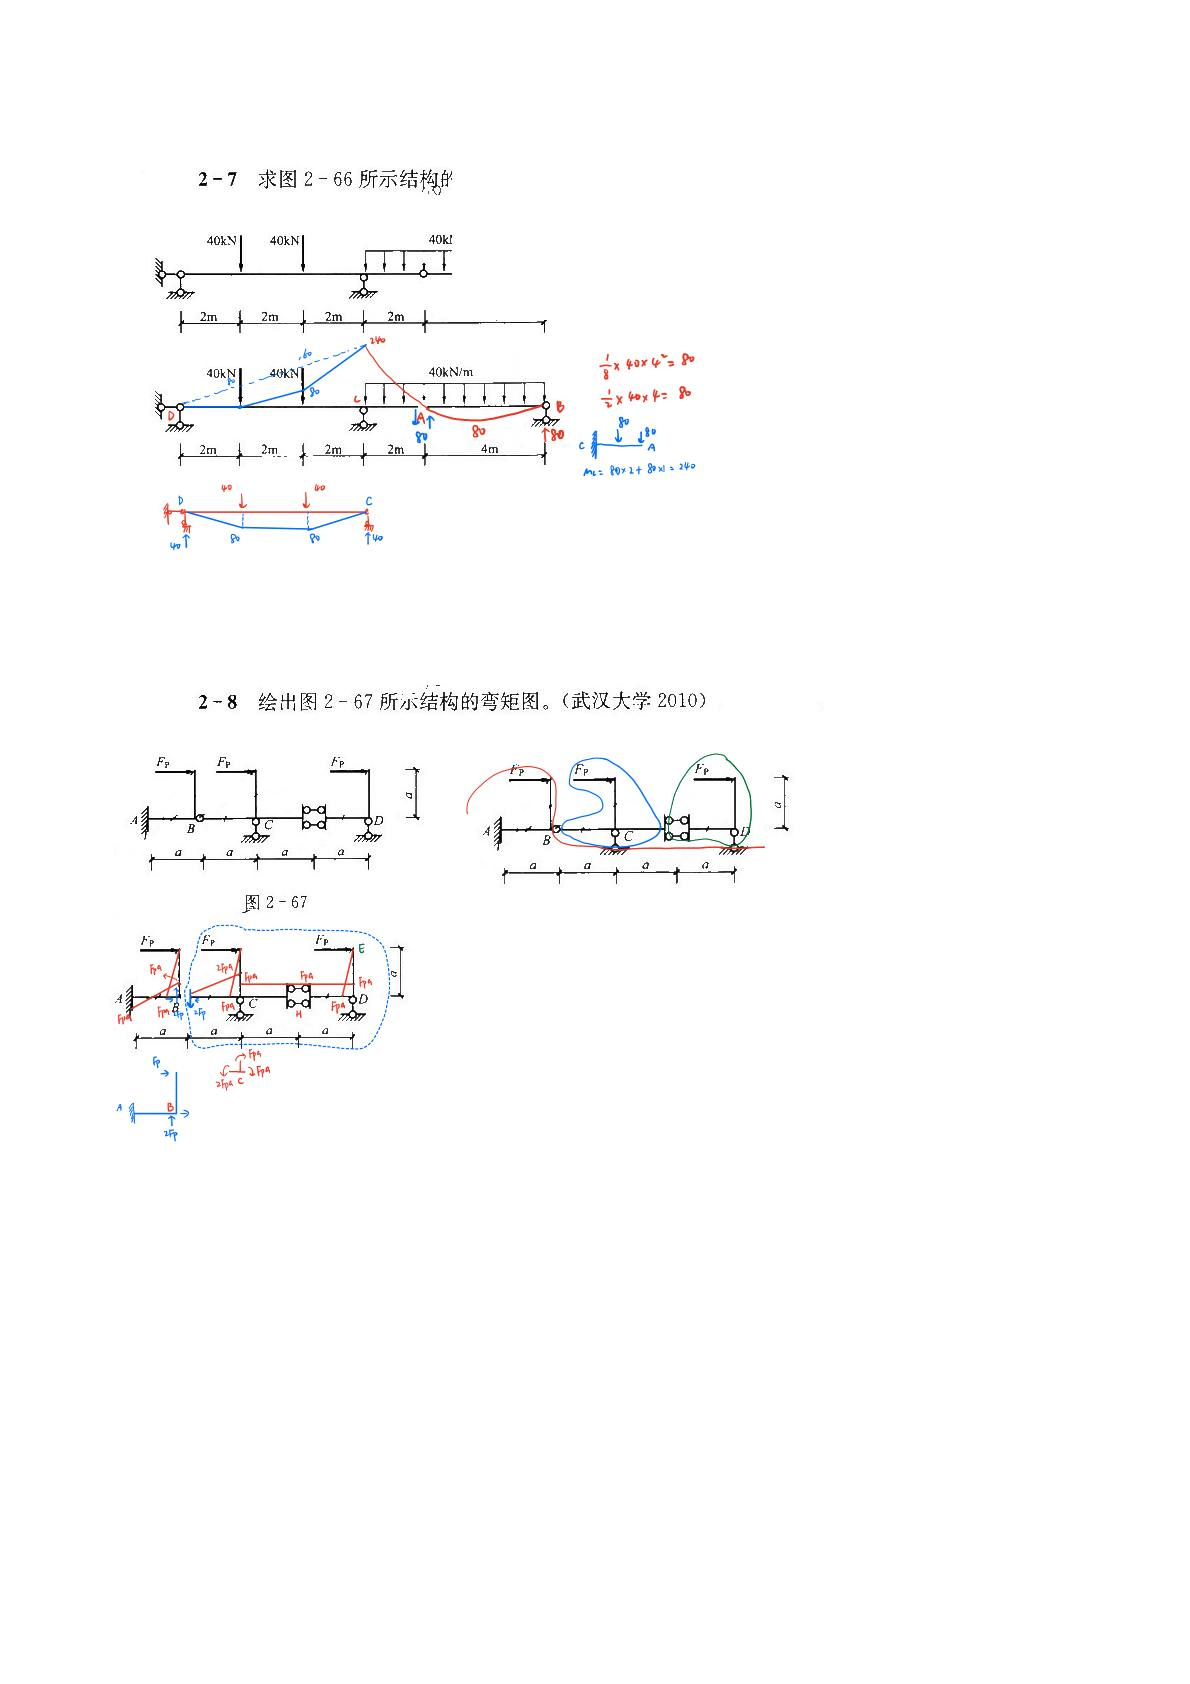
\includegraphics[width=0.92\textwidth]{figures/src24_p004.jpg}
\caption{【第4次作业笔记】 梁和刚架(1) 第 4 页清理图形页}
\end{figure}
\subsection*{第 5 页转写}
2-g作图2-68所示静定刚架M图。（福州大学2008）

MD+4x / -3$\times$2=0

Mp= 2

3kN-m

2m

图2-68

EMg=0

绘制图2-69所示结构的弯矩图。（武汉科技大学20Q9）

Z-10

\$t=,t x01x

K=0M=C

102/m

20kN

165

13120

Fap=40

3F80+

10$\times$3$\times$15 = 16t

3m

3m

3m

图2-69
\begin{figure}[H]\centering
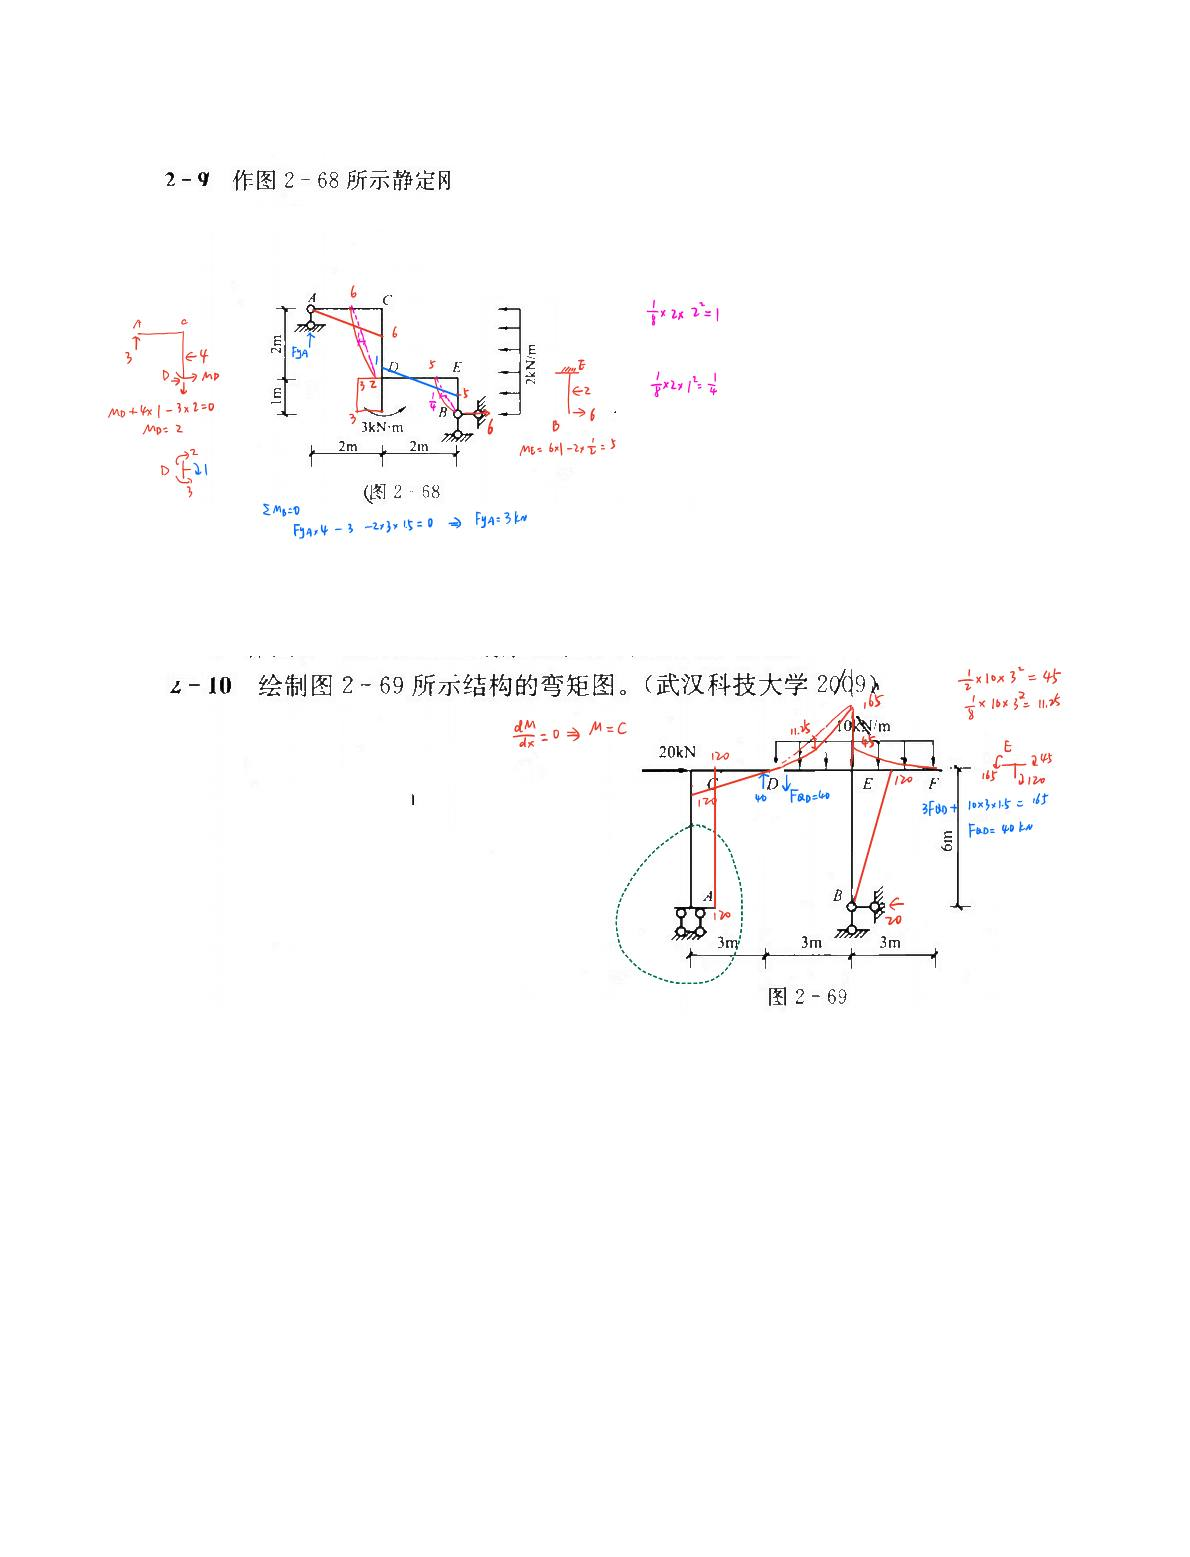
\includegraphics[width=0.92\textwidth]{figures/src24_p005.jpg}
\caption{【第4次作业笔记】 梁和刚架(1) 第 5 页清理图形页}
\end{figure}
\subsection*{第 6 页转写}
2-11绘图2-70所示结构的弯矩图。（重庆大学2012）

Focrl- 9lx -9t

 + Fo

/2-12已知图2-71所示结构的弯矩图，试作剪力图和轴力图。已知Fp=10kN，M=

40kN m。（哈尔滨工业大学2010）

40

20

20

10kv

10=Fp

M图(kN m)

Q图

20

2m

2m

图2-7

10

N图
\begin{figure}[H]\centering
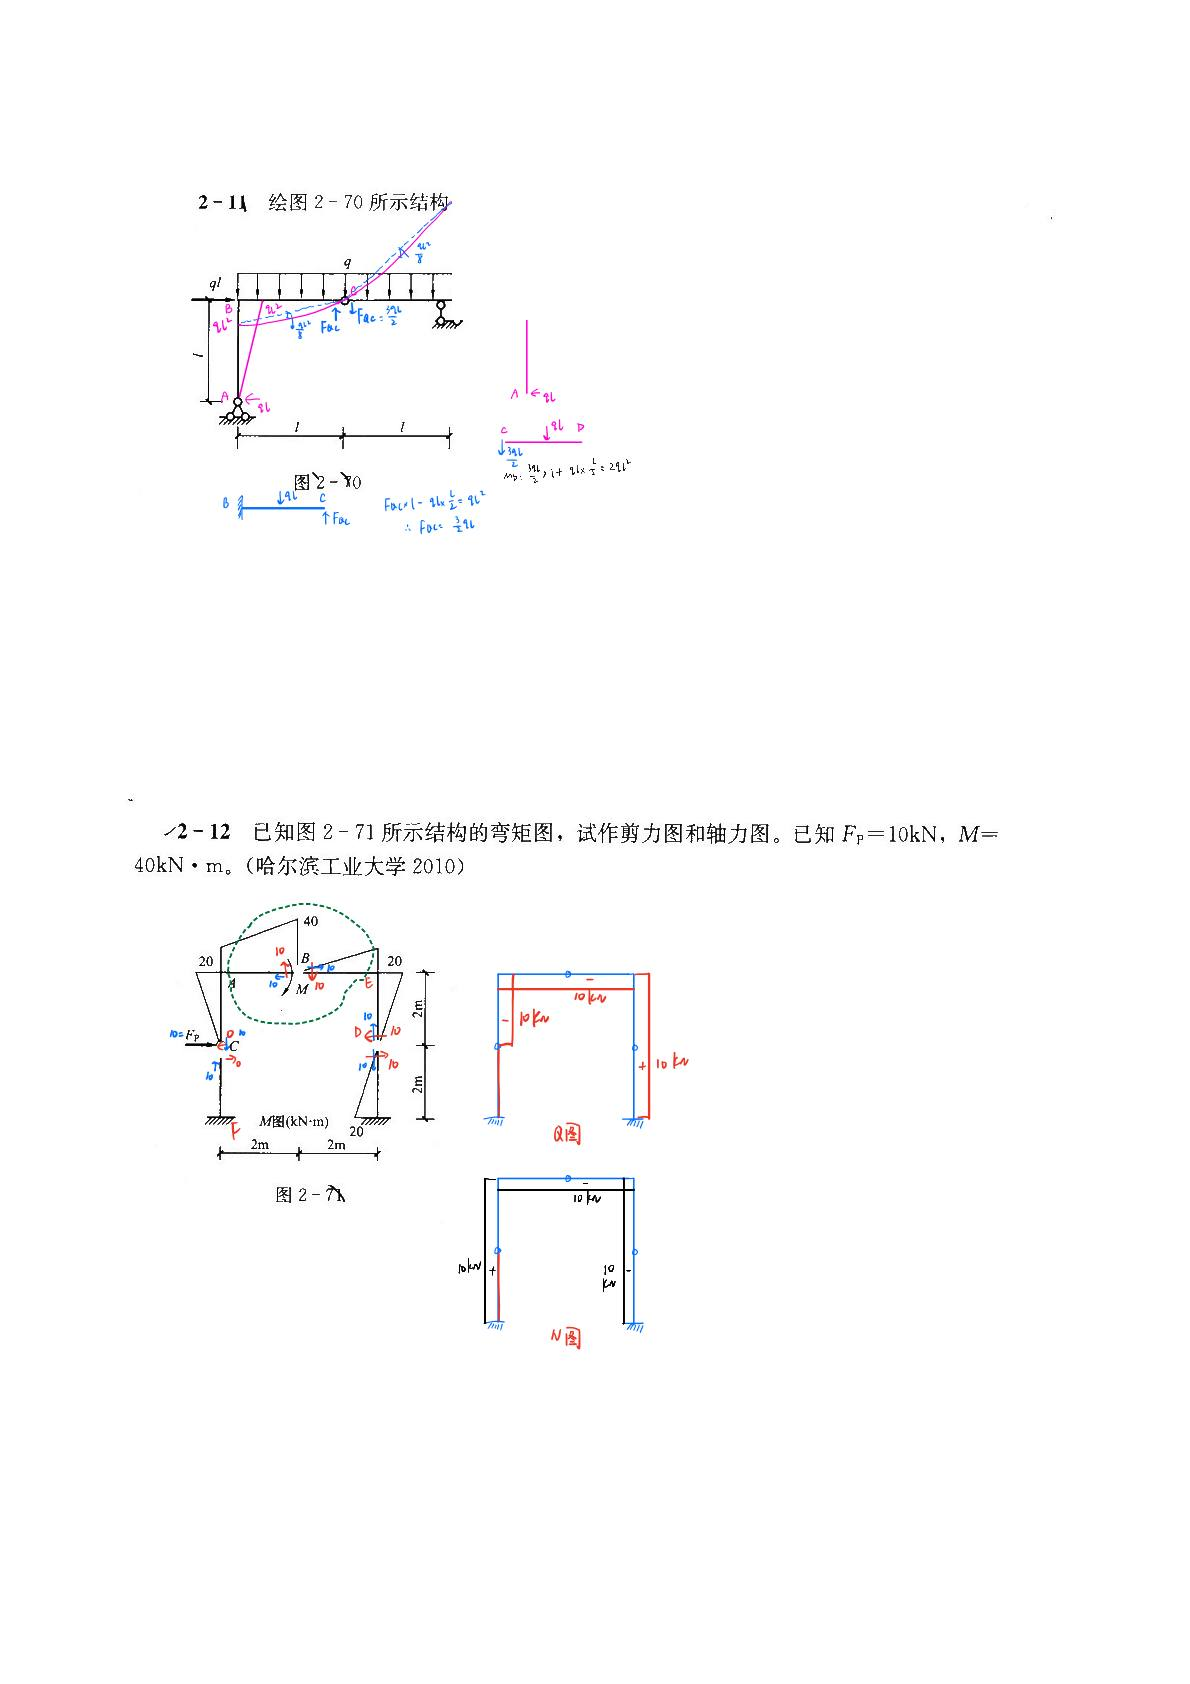
\includegraphics[width=0.92\textwidth]{figures/src24_p006.jpg}
\caption{【第4次作业笔记】 梁和刚架(1) 第 6 页清理图形页}
\end{figure}
\subsection*{第 7 页转写}
2-13

作图2－72所示刚架的弯矩图。（中南大学2009）

0- 2?

ME+ alx

291

图2-72

" ME-

2 - 14

绘出图2－73所示结构的弯矩图。（武汉大学2010）

2kN/m 4

4kN-m

=M=C

3m

2kN/m

4kN-m

3kN

图2-73

ME

Mob -2x2*1 -4= 0

ZME=0, 8+ ME-7+4=D, ME:7o
\begin{figure}[H]\centering
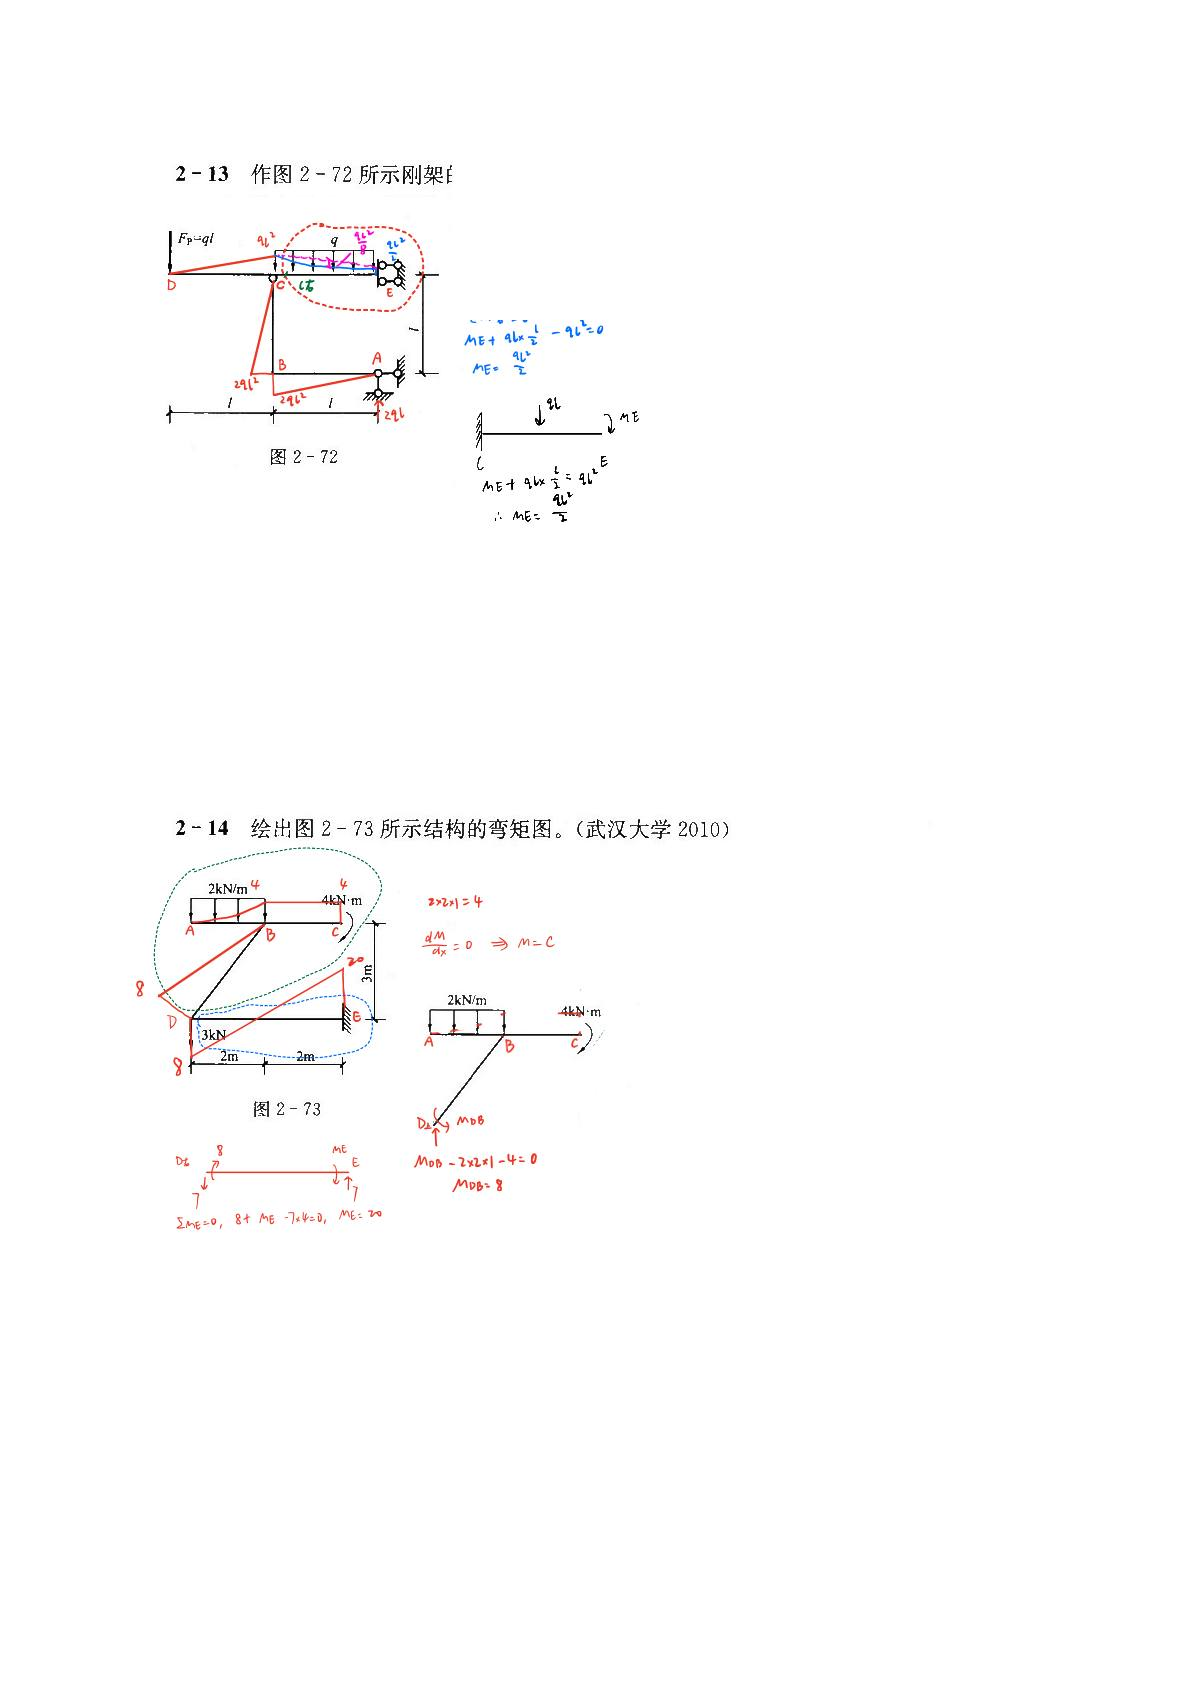
\includegraphics[width=0.92\textwidth]{figures/src24_p007.jpg}
\caption{【第4次作业笔记】 梁和刚架(1) 第 7 页清理图形页}
\end{figure}
\subsection*{第 8 页转写}
2 -15

作图2-74所示结构的内力图。（北京工业大学2011)

30kN-m

内力图是指弯矩图，剪力图及轴力图。

10kN

170

30kN

170-o

8m

2m

2m

m (Nw)

+T40

图2-74

1485

30kN-m

30kN-m

10kN

4m

10kN

518

30kN

30kN

10kN/m

815

9875

8m

8m

(m)

2 -16

求图2－75所示结构的内力，并作弯矩图。（可不写过程）（东南大学2008）

Fpa

图2-75

Fpa

Fpa

4$\times$ Fpp 24
\begin{figure}[H]\centering
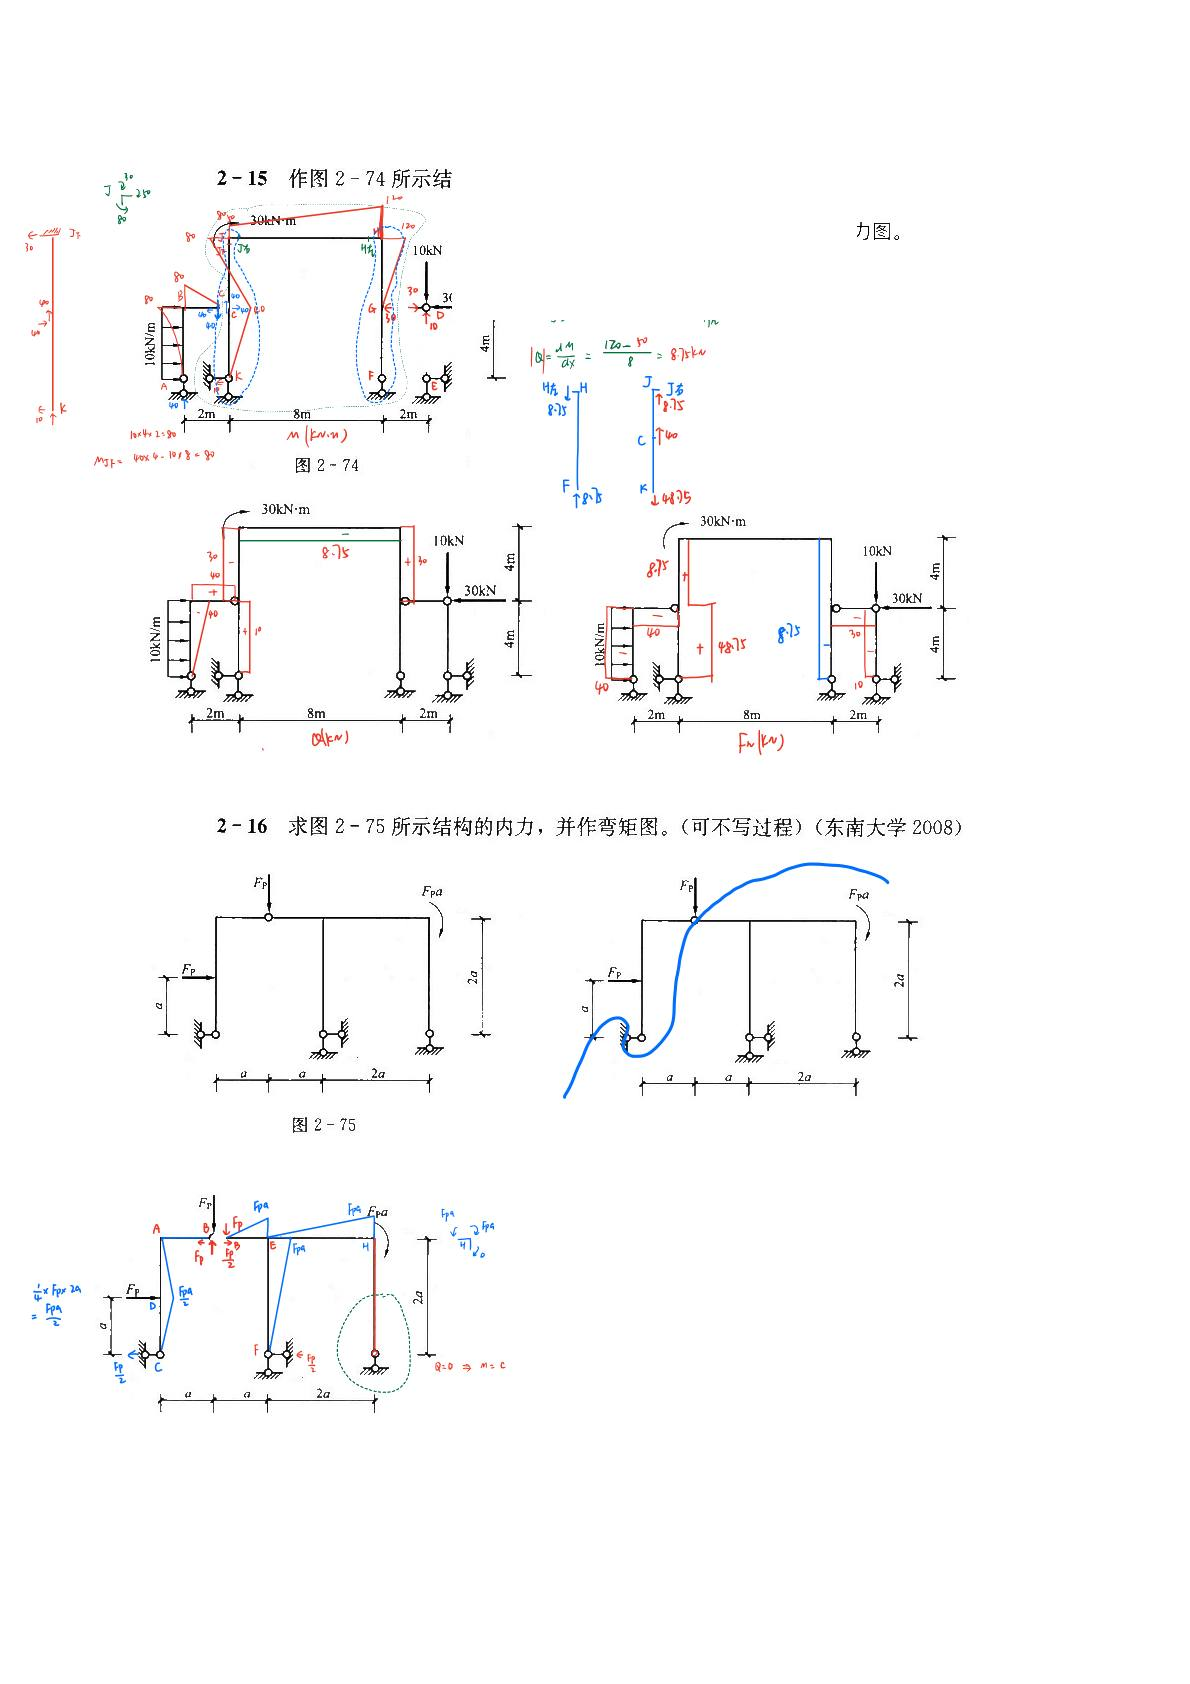
\includegraphics[width=0.92\textwidth]{figures/src24_p008.jpg}
\caption{【第4次作业笔记】 梁和刚架(1) 第 8 页清理图形页}
\end{figure}
\subsection*{第 9 页转写}
2-17

作图2－76所示结构的弯矩图。（无须写出分析过程）（东南大学2007）

20kN/m

10kN/m

6m

6m

图2-76

5759

20kN/m

20kN/m

EMA:0

675

1525

2hj8- box-30x75- 2ex 12 6=D

4.15

6m

mhz 7ox6x3- 4875x 6s 675

2 - 18

作图2-77所示结构弯矩图。（中南大学2010)

10kN/m

10kN/m

30kN

30kN

40kN

40KN

2m

图2-次

10kN/m

ZMA=0

. Fx6-73
\begin{figure}[H]\centering
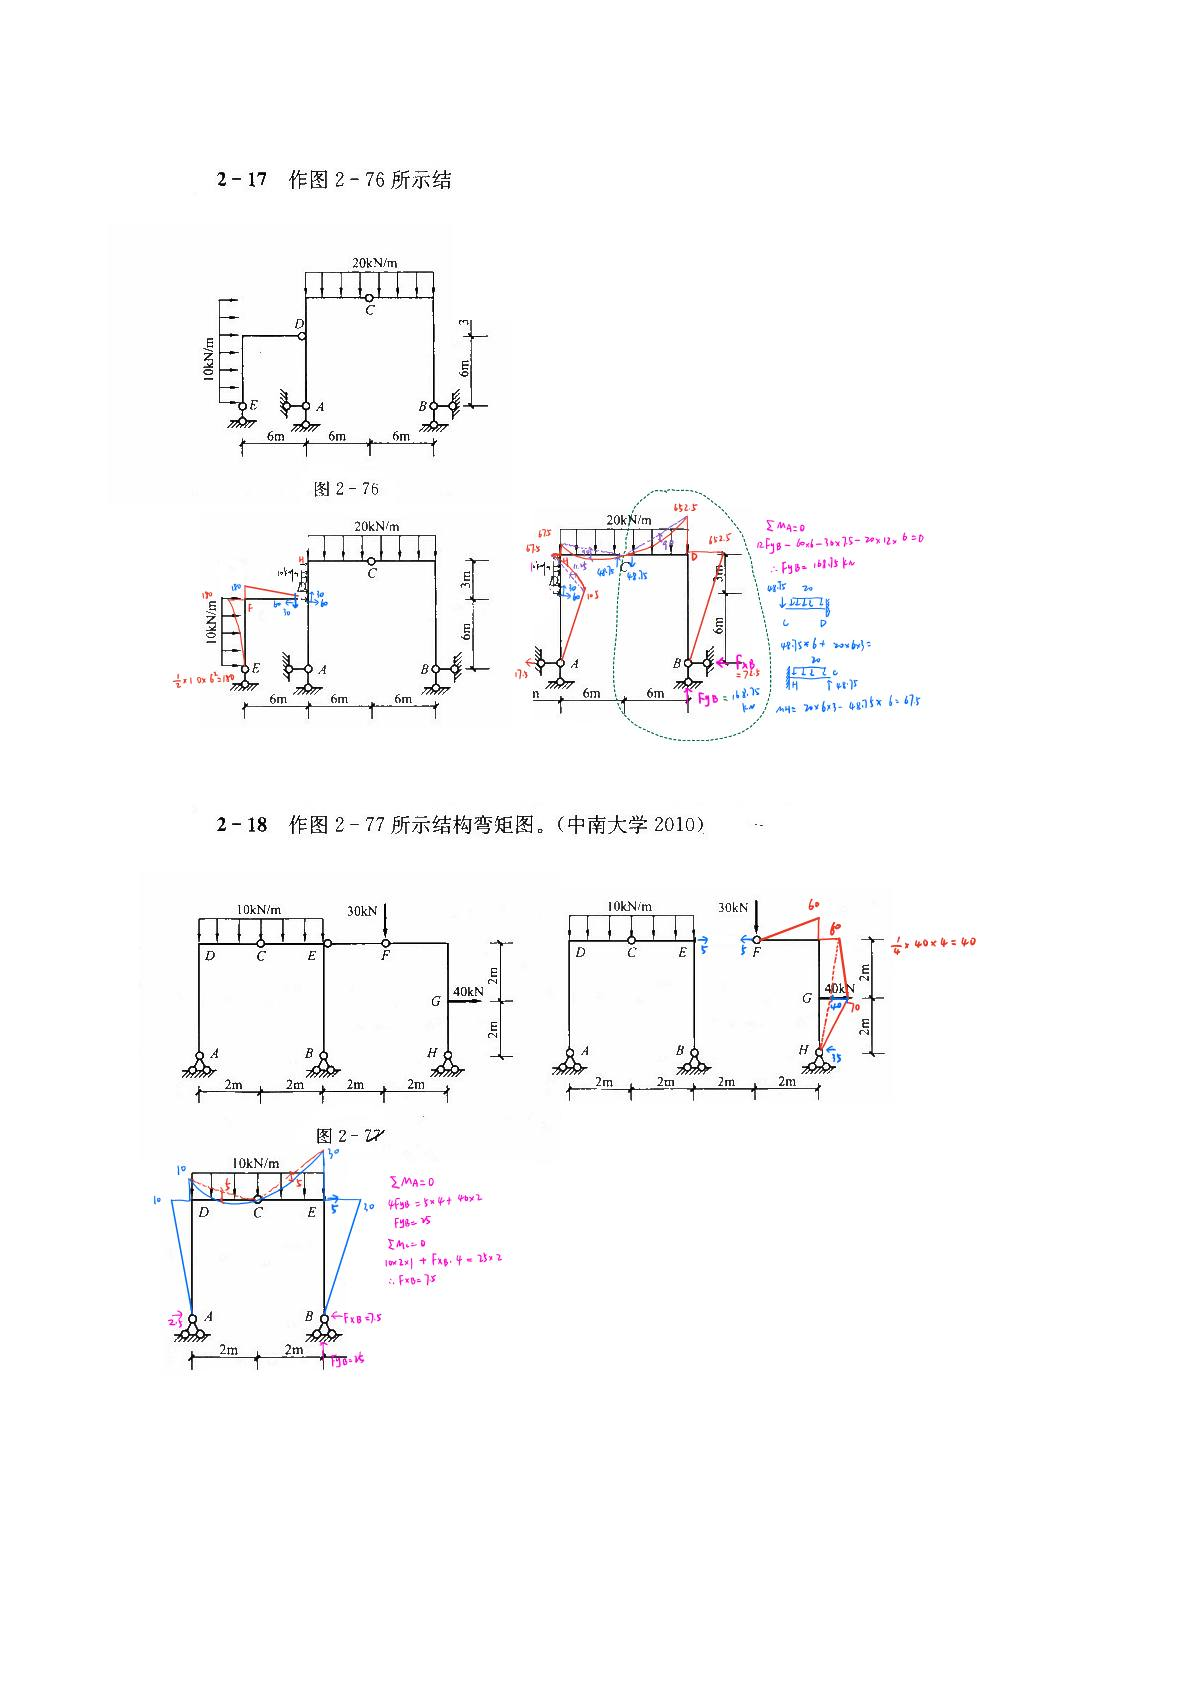
\includegraphics[width=0.92\textwidth]{figures/src24_p009.jpg}
\caption{【第4次作业笔记】 梁和刚架(1) 第 9 页清理图形页}
\end{figure}
\subsection*{第 10 页转写}
2-19已知结构在集中力和集中力偶矩作用下的弯矩图如图2-78所示，其中BC段

为二次抛物线，试确定结构所受的荷载情况，并绘出BE段隔离体受力平衡图。（北京交通

大学2009)

81-29

BC23941

2qd

F-b

E$\times$ 24 =30A2

294

344

2a

24$\times$ 4$\times$ 2+ BE$\pm$4= 394t

. 0E- 214

图2-78

2-20已知图2-79所示静定刚架的弯矩图（曲线部分为二次抛物线），试绘图标出作

用于刚架上的荷载，并作出剪力图和轴力图（假设各杆无局部平衡的轴向荷载，无分布力

偶）。（浙江大学2012）

3.3INI

ME= FxB-4- 2x++2- 2

. Fxbe 45

M图(kNm)

FxB=45

2m

2m

79

N K\textasciitilde{})
\begin{figure}[H]\centering
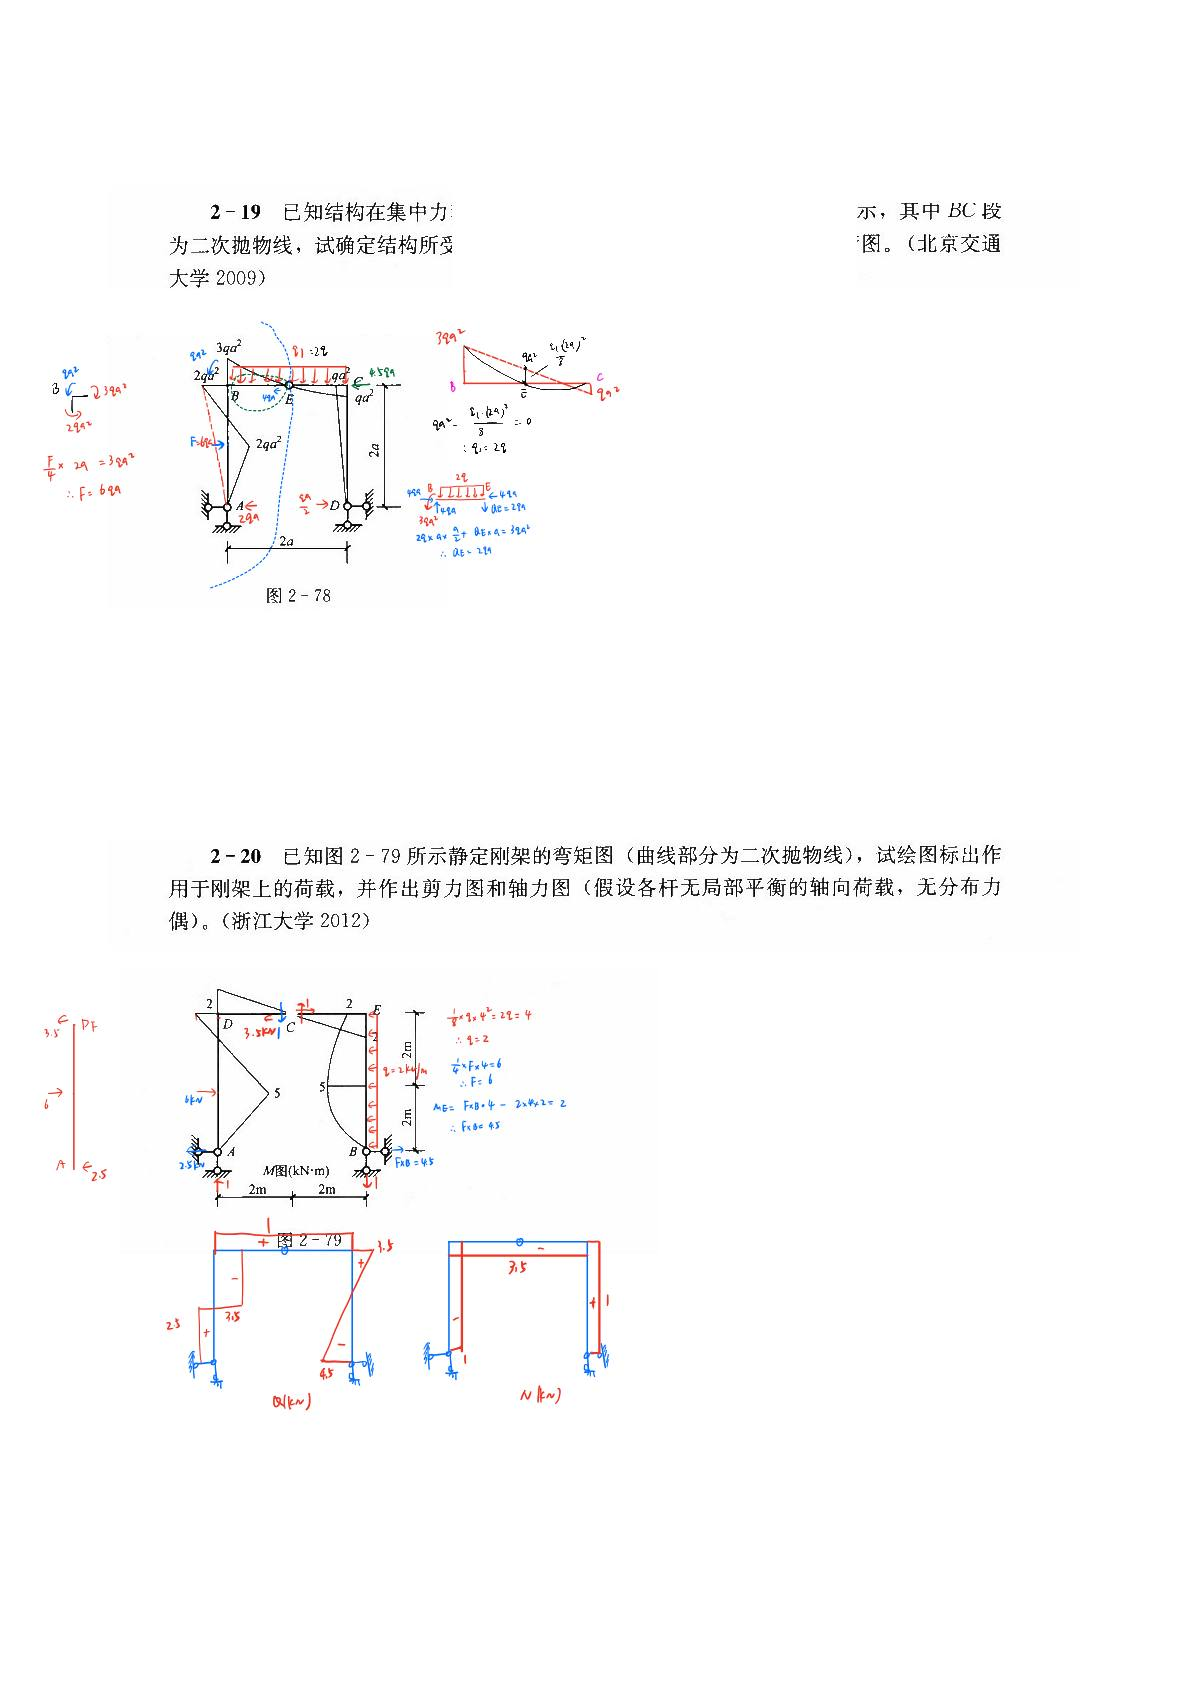
\includegraphics[width=0.92\textwidth]{figures/src24_p010.jpg}
\caption{【第4次作业笔记】 梁和刚架(1) 第 10 页清理图形页}
\end{figure}
\subsection*{第 11 页转写}
2-21不经过计算，绘制图2-80所示结构弯矩图。（武汉科技大学2009）

10kNm

Q=CM斜直缘

5m

图2-80

2-22

试求解图2-81所示刚架，并绘制弯矩图。（东北大学2005）

反对称荷载下，弯矩图和轴力图是反对称的，

剪力图是正对称的。

J=WE0=0

AFP

3m

3m

3m

3m

图2-8Y
\begin{figure}[H]\centering
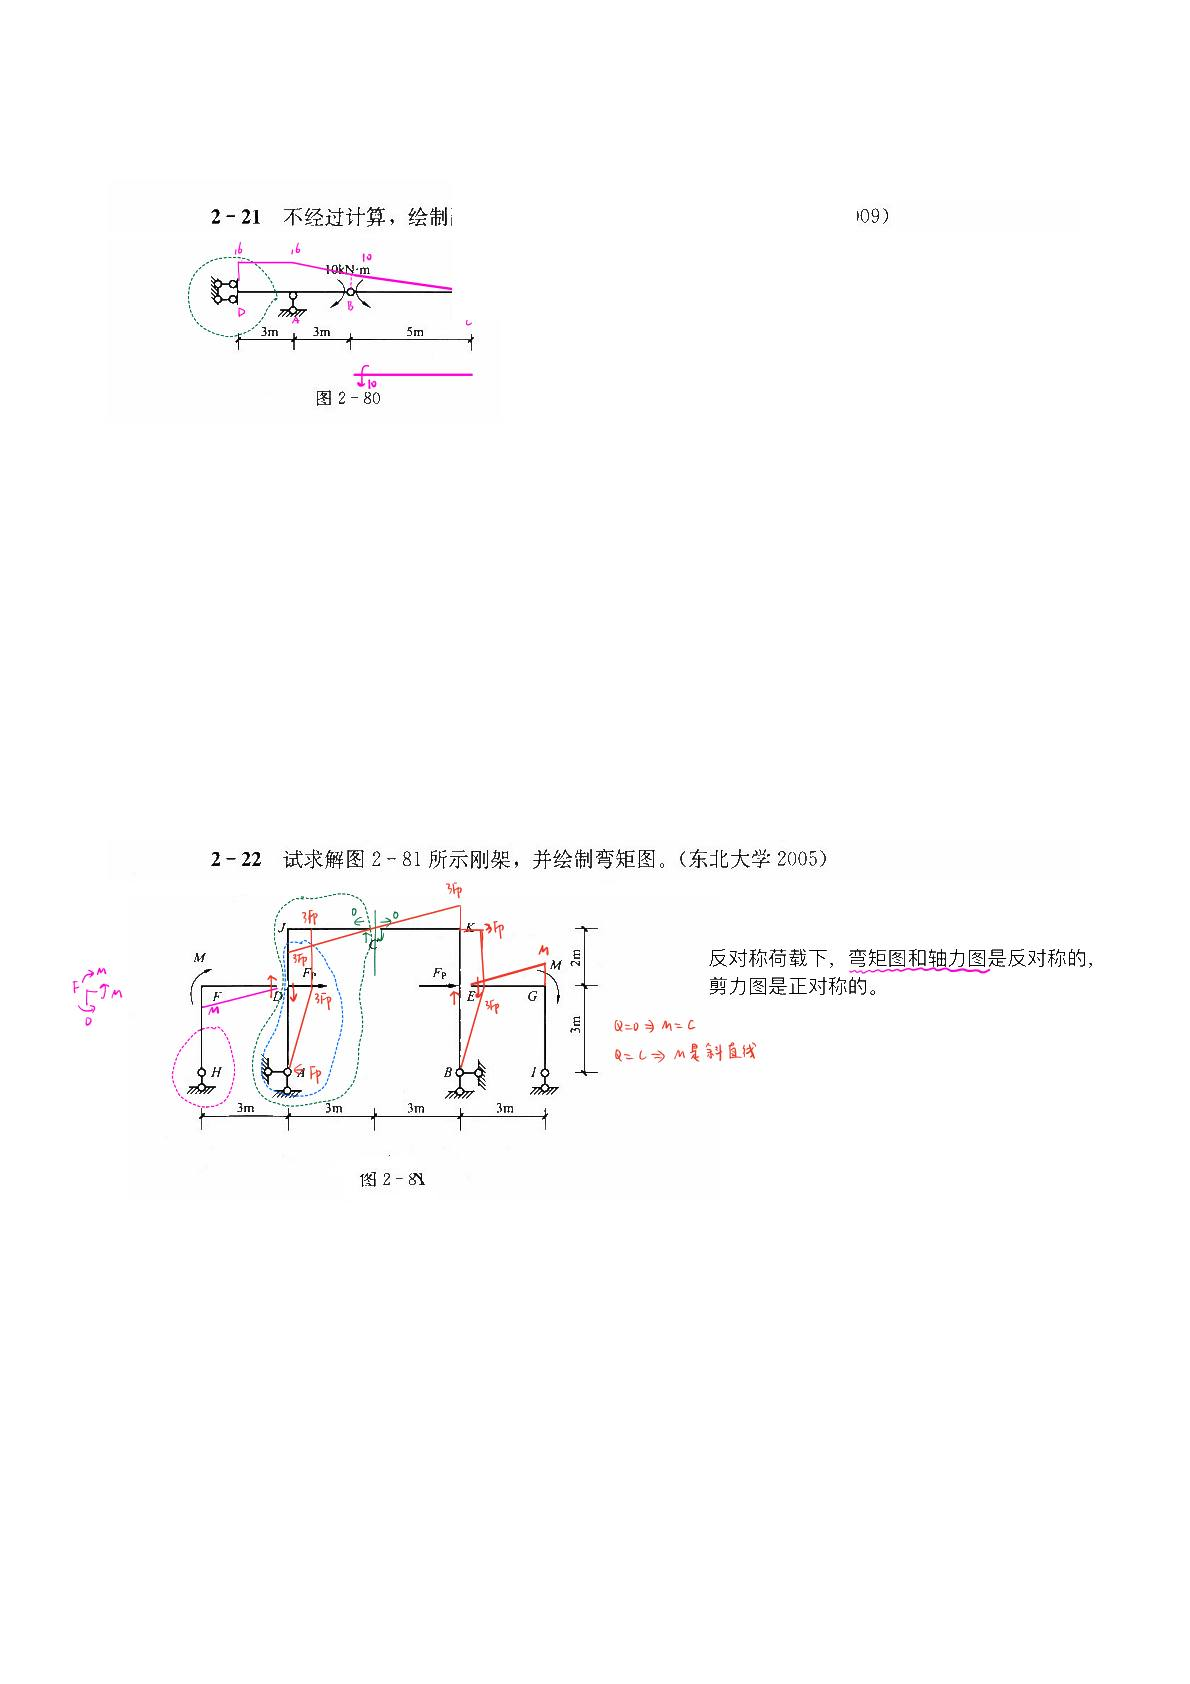
\includegraphics[width=0.92\textwidth]{figures/src24_p011.jpg}
\caption{【第4次作业笔记】 梁和刚架(1) 第 11 页清理图形页}
\end{figure}
